\documentclass{article}
\usepackage{amsmath}
\usepackage{amssymb}
\usepackage[page,toc,titletoc,title]{appendix}
\usepackage{authblk}
\usepackage{bbold}
\usepackage[backend=biber,style=alphabetic,sorting=ynt]{biblatex}
\usepackage{float}
\usepackage{msc}
\usepackage{graphicx}
\usepackage{minted}
\usepackage[skip=7pt plus1pt, indent=20pt]{parskip}
\usepackage{physics}
\usepackage{svg}
\usepackage{tikz}
%\usepackage{tikz-3dplot}
%\usetikzlibrary{3d}          
%\usetikzlibrary{perspective} 
\usetikzlibrary{quantikz}
\usepackage{xurl}
\addbibresource{bibliography.bib}

\begin{document}

\begin{titlepage}
   \begin{center}
       \vspace*{1cm}

       \Large
       \textbf{Simulation of a quantum communication protocol in prepare-and-measure and entanglement scenarios}

       \vspace{0.8cm}

       \normalsize
       \textbf{Aido Cort\'es Alcar\'az, I\~{n}aki Ortiz de Landaluce S\'aiz and Tom\'as Albert Pastor Juro}

       \vfill
            
       \footnotesize{A project submitted for the Postgraduate Degree in Quantum Engineering}
            
       
\includegraphics[width=0.8\textwidth]{images/upc.png}
            
       \date{\today}
            
   \end{center}
\end{titlepage}
\newpage
\renewcommand{\abstractname}{Abstract}
\begin{abstract}
In the early years of the current century, a breakthrough was made in Quantum Information theory by David Bacon and Ben Toner, who developed a quantum communication protocol showing that any prediction based on projective measurements (PVMs) on a qubit could be simulated by communicating only two classical bits. This result has been very recently extended by Martin Renner, Armin Tavakoli and Marco Tulio Quintino to positive operator-valued measures (POVMs) without any loss of generalisation and classical cost of a qubit transmission, still two bits. In this project we have simulated such extended protocol both classically and using a quantum computing framework, to show how two bits of communication are enough to reproduce all quantum correlations associated to arbitrary POVMs applied to any prepare-and-measure scenario and also to any entangled two-qubit state. With this investigation we give rise to explore and understand computationally the fundamental limits of quantum over classical advantages.
\end{abstract}
\newpage
\tableofcontents

\newpage
\section{Introduction}
\subsection{Objective}
Quantum information theory provides a framework to quantify the power of quantum theory compared to Shannon's classical communication theory \cite{shannon}. Over the last decades, the field has flourished compelled to set realistic boundaries to the promises of quantum advantages in fields like quantum communication and computing. An important feature of quantum theory lies in the statistical correlations produced by local measurements of a quantum system. The simplest example of quantum correlations are the ones produced by projective measurements on a maximally-entangled state of two qubits, also known as a Bell pair state. Such correlations are the basic resource of bipartite quantum information theory, where various equivalences are known: one shared Bell pair plus two bits of classical information can be used to teleport one  qubit and, conversely, one shared Bell pair state plus a single qubit can be used to send two bits of classical information via superdense coding. Exploring the fundamental limits of quantum over classical advantages in these scenarios is crucial, and it will be the primary objective of this work.
\par
In the early years of the current century, Ben Toner and David Bacon developed a protocol which proves that any prediction based on projective measurements on an entangled Bell pair state could be simulated by communicating only two classical bits \cite{toner2003}. Very recently, Martin Renner, Armin Tavakoli and Marco Tulio Quintino, have extended such result to a most generalised set of measurements, the positive operator-valued measures \cite{renner2022}.
Following up such generalization, we will show via classical and quantum computer-based experiments that a qubit transmission can be simulated classically with a total cost of two bits for any general measurement, either in a prepare-and-measure or an entanglement scenario. This will prove experimentally that the protocols described in \cite{renner2022} can be reproduced computationally using classical computers and quantum simulators.
\par
Before starting to describe the different computational experiments we have carried out to achieve such goal, it is worth spending next sections to introduce some preliminary concepts and notations that have been used extensively throughout this work, specifically the definition of positive operator-valued measures, the set-up of both the prepare-and-measure and Bell scenarios and the particular details of the classical simulation protocols applied to such scenarios.
\par
\subsection{Positive operator-valued measures}\label{section:povms}
Even when most of the introductory textbooks on quantum mechanics describe the measurement postulates using projective measurements only, there exists a more general and less restrictive set of measurements called Positive Operator-Valued Measures or POVMs, see \cite{nielsen2000}\cite{peres1995}. The underlying formalism behind POVMs is uniquely well adapted for some applications where the main focus is on describing the probabilities of the different measurement outcomes rather than on the post-measurement state of the system. This is of particular interest in quantum communication and quantum information, where a more comprehensive formalism for the description of the measurements is needed, and highlights how important are the results from \cite{renner2022}, where all the results are extended to POVMs without any loss of generalisation regarding the the classical simulation cost of the protocol. For reference, we define explicitely a POVM as a set $\mathbb{P}_N=\{B_b\}$ of $b=1,...,N$ positive semidefinite operators acting on a Hilbert space $\mathcal{H}$ of dimension $d_{Q}$, which satisfies the closure property $\sum_{b=1}^{N} B_{b} = \mathbb{1}$. The operator $B_{b}$ is called a POVM element, and it is associated to the outcome $b$ of the POVM. In this work we will use extensively the property which states that every qubit POVM can be written as a coarse graining of rank-1 projectors \cite{barrett2002}, such that we will restrict our POVM calculations to the case of rank-1 projectors.

\subsection{Prepare-and-measure scenario}\label{section:pm}
As for many other communication protocols we have two well-known characters playing different roles in the quantum prepare-and-measure set-up: Alice and Bob. The prepare-and-measure scenario starts with Alice preparing a random quantum state and sending it to Bob. In a general set-up, i.e. not restricted to single qubit communication, the state prepared by Alice is a state of dimension $d_Q$ described by a positive semidefinite density matrix $\rho \in \mathcal{L}( \mathbb{C}_{d_Q}), \rho \ge 0$ with unit trace $tr(\rho)=1$. Once the state is prepared and communicated by Alice, Bob then receives it and performs a random quantum measurement on it, obtaining an outcome $b$. In the case of general POVM measurements $\mathbb P=\{B_b\}$ as described in Section \ref{section:povms}, the probability of outcome $b$ when performing the measurement on the state $\rho$ is given by Born's rule,

\begin{equation}\label{eq:prob_quantum}
p_Q(b|\rho,\{B_b\}) = tr(\rho B_b)
\end{equation}

In the context of this work, we are interested in the classical counterpart of the quantum prepare-and-measure scenario, where the probability distributions predicted by the quantum theory (\ref{eq:prob_quantum}) are reproduced classically. All these classical counterparts of existing quantum protocols, see examples in \cite{cerf2000}, \cite{toner2003} and \cite{renner2022}, require a shared randomness $\lambda$ among Alice and Bob subject to some probability function $\pi(\lambda)$ to correlate their classical communication strategies. As it is not possible to reproduce these correlations without communication, a classical message $c$ which encodes classically the quantum state $\rho$ taking its value from a $d_C$-valued alphabet $\{1,...,d_C\}$ is also required. Alice's actions are therefore described by the conditional probability $p_A(c|\rho,\lambda)$, whereas Bob's actions are similarly described by the conditional probability $p_B(b|\{B_b\},c,\lambda)$. If we consider both probabilities, the correlations from the classical counterpart become

\begin{equation}\label{eq:prob_classic}
p_C(b|\rho,\{B_b\}) = \int_{\lambda} d\lambda\ \pi(\lambda) \sum_{c=1}^{d_C} p_A(c|\rho, \lambda) p_B(b|\{B_b\}, c, \lambda)
\end{equation}

Given Equation (\ref{eq:prob_quantum}) and (\ref{eq:prob_classic}), the classical simulation would be considered successful when, for every random state and POVM, the classical probability distribution reproduces the quantum predictions, i.e.

\begin{equation}\label{eq:prob_classic_quantum}
\forall \rho, \{B_b\}:\quad p_C(b|\rho,\{B_b\}) = p_Q(b|\rho,\{B_b\})
\end{equation}

\subsection{Bell scenario}
In a Bell scenario, there is a bipartite quantum system of two entangled and separated qudits, one with Alice and another one with Bob. 
Alice chooses a random local measurement, and produces an output according to the distribution of her measurement elements. Following the same procedure, Bob chooses his own random local measurement and produces an outcome. Even if both outcomes appear random, their joint probabilities are correlated. We refer to these correlations as Bell correlations.

Similarly to the prepare-and-measure case described in Section \ref{section:pm}, it is not possible to reproduce the correlations using a classical protocol with shared random variables without allowing classical communication among Alice and Bob once they have selected their measurements, see \cite{bell1964}. The main question here is to determine how much classical communication is needed to reproduce the probability distributions.

As \cite{renner2022} shows, it is straight-forward to adapt the prepare-and-measure classical scenario to any entangled qudit-qubit state. Here Alice chooses a random local POVM on a $d_Q$-dimensional quantum system, and produces an output according to the marginal distribution of her POVM elements. Based on her output, she computes Bob's entangled qubit post-measurement state, which is sent to Bob using the prepare-and-measure scenario. Given that Bob's post-measurement qubit state is communicated by Alice using the existing prepare-and-measure classical protocol, the classical cost of the qubit transmission will be exactly the same. 

In addition to this, we will discuss in the next sections other Bell scenarios where the entangled state is a Bell singlet state and the classical simulation cost is reduced to one bit.


\subsection{Classical simulation protocols}\label{section:protocols}
\subsubsection{Prepare-and-measure with one qubit}\label{section:protocol_pm}
The classical prepare-and-measure protocol proposed by Renner, Tavakoli and Quintino \cite{renner2022} is restricted to qubits ($d_Q=2$), and makes an extensive use of the geometrical properties of a qubit state in the Bloch sphere. Since mixed qubit states are convex combinations of pure states, the protocol is also restricted to the usage of pure states only. Toner and Bacon proved that making a further restriction to projective measurements, i.e. $B_b^{2} = B_b$, the classical simulation cost was upper bounded by two classical bits ($d_C=2$) \cite{toner2003}, but \cite{renner2022} generalizes the results to positive operator-valued measures with a minimal and therefore necessary classical cost of two qubits. Finally, the protocol is also restricted without any loss of generality to POVMs proportional to rank-1 projectors, following results in \cite{barrett2002}.

In Bloch notation, qubit states $\rho$ are represented by three-dimensional real normalized vectors $\vec{x} \in \mathbb{R}^{3}$, and rank-1 POVM projectors as $B_b = 2p_b\ket{\vec{y}_b}\bra{\vec{y}_b}$, where $p_b\ge0,\ \sum_{b=1}^{N}p_b=1$ and $\ket{\vec{y}_b}\bra{\vec{y}_b} = \frac{\mathbb{1} + \vec{y}_b \cdot \vec{\sigma}}{2}$ for some normalized vector $\vec{y}_b \in \mathbb{R}^{3}$, such that

\begin{equation}
tr(\rho B_b) = p_b(1 + \vec{x} \cdot \vec{y}_b) 
\end{equation}

Two additional functions need to be defined prior to make the classical protocol steps explicit, these are the Heaviside function
\begin{equation}
H(z) =
    \begin{cases}
      1 & \text{when $z \ge 0$}\\
      0 & \text{when $z<0$}
    \end{cases} 
\end{equation}
and $\Theta(z) := z \cdot H(z)$. Under all these considerations, the protocol, as defined in \cite{renner2022} and sketched in Figure \ref{fig:msc_pm}, is literally as follows:
\begin{enumerate}
 \item Alice and Bob share two normalized vectors $\vec{\lambda}_1, \vec{\lambda}_2 \in \mathbb{R}^{3}$, which are uniformly and independently distributed on the unit radius sphere $S_2$.
 \item Instead of sending a pure qubit $\rho = (\mathbb{1} + \vec{x} \cdot \vec{\sigma})/2$, Alice prepares two bits via the formula $c_1= H(\vec{x} \cdot \vec{\lambda}_1)$ and $c_2= H(\vec{x} \cdot \vec{\lambda}_2)$ and sends them to Bob.
 \item Bob flips each vector $\vec{\lambda}_i$ when the corresponding bit $c_i$ is zero. This is equivalent to set $\vec{\lambda}^{\prime}_{i} := (-1)^{1 + c_i} \vec{\lambda}_{i}$.
 \item Instead of performing a POVM with elements $B_b = 2p_b\ket{\vec{y}_b}\bra{\vec{y}_b}$, Bob picks one vector $\vec{y}_b$ from the set $\{\vec{y}_b\}$ according to the probabilities $\{p_b\}$. Then he sets $\vec{\lambda} := \vec{\lambda}^{\prime}_1$ if $\lvert \vec{\lambda}^{\prime}_1 \cdot \vec{y}_b \rvert \ge \lvert \vec{\lambda}^{\prime}_2 \cdot \vec{y}_b \rvert$ and $\vec{\lambda} := \vec{\lambda}^{\prime}_2$ otherwise. Finally, Bob outputs $b$ with probability
\end{enumerate}

\begin{equation}\label{eq:prob_classic_bob}
p_B(b|\{B_b\},\vec{\lambda}) = \frac{p_b\ \Theta(\vec{y}_b \cdot \vec{\lambda})}{\sum_{j}^{N}p_j\ \Theta(\vec{y}_j \cdot \vec{\lambda})}
\end{equation}

\begin{figure}[tb]
\begin{center}
\begin{msc}[msc keyword=, instance width=3.6cm]{Prepare-and-measure classical protocol}
\declinst{alice}{}{Alice}
\declinst{bob}{}{Bob}
\condition*{shared randomness $\vec{\lambda}_1, \vec{\lambda}_2$}{alice,bob}
\nextlevel[3]
\action*{$c_i = H(\vec{x} \cdot \vec{\lambda_i})$}{alice}
\nextlevel[3]
\mess{$c_1, c_2 \in \{0,1\}$}{alice}{bob}
\nextlevel[1]
\action*{$\vec{\lambda}^{\prime}_i = (-1)^{1 + c_i} \vec{\lambda_i}$}{bob}
\nextlevel[3]
\action*{$p_B(b|\{B_b\},\vec{\lambda})$}{bob}
\nextlevel[2]
\end{msc}
\end{center}
\caption{Classical prepare-and-measure protocol sequence: Alice sends two bits $c_1, c_2$ resulting from projecting the qubit state's Bloch vector $\vec{x}$ with respect to the shared random vectors $\vec{\lambda}_1, \vec{\lambda}_2$ through a classical channel, Bob flips the shared random vectors when necessary, and finally computes classical probability outcomes according to Equation \ref{eq:prob_classic_bob}.}
\label{fig:msc_pm}
\end{figure}

%https://tex.stackexchange.com/questions/368604/how-to-draw-a-half-and-half-colored-circle
%\pgfmathsetmacro{\radius}{2}
%\begin{tikzpicture}
%    %\fill[gray!50,opacity=0.7] (0,0) circle (\radius); 
%    %\fill[gray!10, opacity=1] (0,0) -- (135:\radius) arc (135:315:\radius) -- cycle; 
%    \draw[] circle(\radius);
%    \draw[thick,->] (0,0,0) -- (\radius,0,0) node[anchor=north west]{$\vec{\lambda}_1$};
%    \draw[thick,->] (0,0,0) -- (-0.3473, 1.9696,0) node[anchor=south east]{$\vec{\lambda}_2$};
%    \draw[thick,->] (0,0,0) -- (1.4142, 1.4142,0) node[anchor=south]{$\vec{x}$};
%    \draw[dashed] (-1.414,1.414,0) -- (1.414,-1.414,0) node[anchor=south]{};    
%\end{tikzpicture}

%\tdplotsetmaincoords{40}{0}
%\tdplotsetrotatedcoords{150}{50}{20}
%\begin{tikzpicture}[scale=2,line join=bevel,tdplot_rotated_coords,fill %opacity=1,declare function={ colorFunc(\t)=ifthenelse(\t>0,60,300);}]
%\pgfsetlinewidth{.0pt}
%    \tdplotsphericalsurfaceplot[parametricfill]{72}{36}{2}%{transparent!0}{colorFunc(180*floor(\tdplotphi/180))
%    }{}{}{}
%\end{tikzpicture}

\subsubsection{Bell with singlet state}\label{section:protocol_bell}
Toner a Bacon showed in \cite{toner2003} that only a single bit was required to classically simulate local projective measurements on a qubit pair in a singlet state $\ket{\psi^{-}}=\frac{1}{\sqrt{2}}(\ket{01} - \ket{10})$. Renner, Tavakoli and Quintino again extended such result being Alice restricted to local projective measurements with outcomes $a=\pm 1$, and Bob allowed to perform any arbitrary POVM measure \cite{renner2022}. The steps for this protocol, sketched in Figure \ref{fig:msc_bell}, are the following:
\begin{enumerate}
 \item Alice and Bob share two normalized vectors $\vec{\lambda}_1^{\prime}, \vec{\lambda}_2 \in \mathbb{R}^{3}$, which are uniformly and independently distributed on the unit radius sphere $S_2$.
 \item Instead of performing a measurement with projectors $\ket{\pm\vec{x}}\bra{\pm\vec{x}} = (\mathbb{1} + \vec{x} \cdot \vec{\sigma})/2$, Alice outputs $a = -sgn(\vec{x} \cdot \vec{\lambda}^{\prime}_1)$ and sends the bit $c = sgn(\vec{x} \cdot \vec{\lambda}^{\prime}_1) \cdot sgn(\vec{x} \cdot \vec{\lambda}_2)$ to Bob, where 
 \begin{equation}
sgn(z) =
    \begin{cases}
      1 & \text{when $z \ge 0$}\\
      -1 & \text{when $z<0$}
    \end{cases} 
\end{equation}
 \item Bob flips the vector $\vec{\lambda}_2$ if and only if $c=-1$, i.e. he sets $\vec{\lambda}^{\prime}_{2} := c \vec{\lambda}_{2}$.
 \item Same as step 4 in the previous prepare-and-measure protocol.
\end{enumerate}

\begin{figure}[tb]
\begin{center}
\begin{msc}[msc keyword=, instance width=3.6cm]{Bell with singlet state classical protocol}
\declinst{alice}{}{Alice}
\declinst{bob}{}{Bob}
\condition*{shared randomness $\vec{\lambda}_1^{\prime}, \vec{\lambda}_2$}{alice,bob}
\nextlevel[3]
\action*{$c = sgn(\vec{x} \cdot \vec{\lambda}^{\prime}_1) \cdot sgn(\vec{x} \cdot \vec{\lambda}_2)$}{alice}
\nextlevel[3]
\mess{$c \in \{-1,1\}$}{alice}{bob}
\nextlevel[1]
\action*{$\vec{\lambda}^{\prime}_2 = c \vec{\lambda_2}$}{bob}
\nextlevel[3]
\action*{$p_B(b|\{B_b\},\vec{\lambda})$}{bob}
\nextlevel[2]
\end{msc}
\end{center}
\caption{Classical Bell with singlet state protocol sequence: Alice sends one bit $c$ resulting from projecting the associated projective measurement's Bloch vector $\vec{x}$ with respect to the shared random vectors $\vec{\lambda}_1, \vec{\lambda}_2$ through a classical channel, Bob flips the shared random vectors when necessary, and finally computes classical probability outcomes according to the response function from the prepare-and measure protocol, see Equation (\ref{eq:prob_classic_bob}).}
\label{fig:msc_bell}
\end{figure}

It can be proved that when Alice outputs $a=+1$, $\vec{\lambda}^{\prime}_1$ and $\vec{\lambda}^{\prime}_2$ are distributed on $S_2$ according to $\rho(\vec{\lambda}^{\prime}_i) = H(-\vec{x} \cdot \vec{\lambda}^{\prime}_i)/(2\pi)$, which corresponds to a classical description of Bob's post-measurement state $-\vec{x}$ and, conversely, when Alice outputs $a=-1$, the random vectors are distributed according to a distribution corresponding to Bob's post-measurement state $\vec{x}$, and therefore Bob can apply the same response function as in the prepare-and-measure protocol described in \ref{section:protocol_pm}. 
\newpage
\section{Methodology}
\subsection{State preparation}
In the classical simulations, the state preparation would require to produce a random qubit pure state first, and then to compute the corresponding Bloch vector to be later used by Alice. 

In the prepare-and-measure scenario, Alice uses the Bloch vector representation of the qubit's pure state, and Bob's POVMs,  proportional to rank-1 projectors, are expressed as the outer product of the associated Bloch vectors. In the Bell scenario, Alice also uses the Bloch vector corresponding to the local projective measurement projectors. Given the fact that the classical and quantum probabilities must be equivalent for any state and POVM set, it is therefore of key importance to be able prepare random Bloch vectors uniformly distributed along the unit radius sphere $S_2$. In addition, in all these simulation protocols, Alice and Bob share two normalized vectors $\vec{\lambda}_1, \vec{\lambda}_2 \in \mathbb{R}^{3}$, which must be uniformly and independently distributed on the same unit sphere $S_2$. Hence the randomized Bloch vector preparation is not only the building block for the state preparation, but also plays a critical role in the measurement construction and shared randomness creation.

To produce a random qubit pure state, we should obtain a random unitary matrix and then apply the unitary transformation to the zero qubit state, resembling the time evolution of a qubit from a zero initial state. The random unitary matrix can be generated by just building a matrix of normally distributed complex numbers, and then apply the Gram-Schmidt QR decomposition to orthogonalize the matrix, see \cite{ozols2009}, \cite{zyczkowski1994}. 

The resulting random qubit state distribution could be validated using the corresponding Bloch vector distribution along the unit radius sphere. A tessellation scheme called HEALPix \cite{healpix}, which produces a hierarchical and equal-area iso-latitude pixelation of a sphere, could be used to show that the random Bloch vectors are uniformly and independently distributed in the Bloch sphere. Given that each pixel in HEALPix covers the same surface area as every other pixel (see Figure \ref{fig:healpix_sphere}), we could group the Bloch vector distribution along the different pixel indices (see Figure \ref{fig:healpix_numbering}), and check whether the resulting distribution is uniform as expected.

\begin{figure}[!ht]
\begin{center}
\centerline{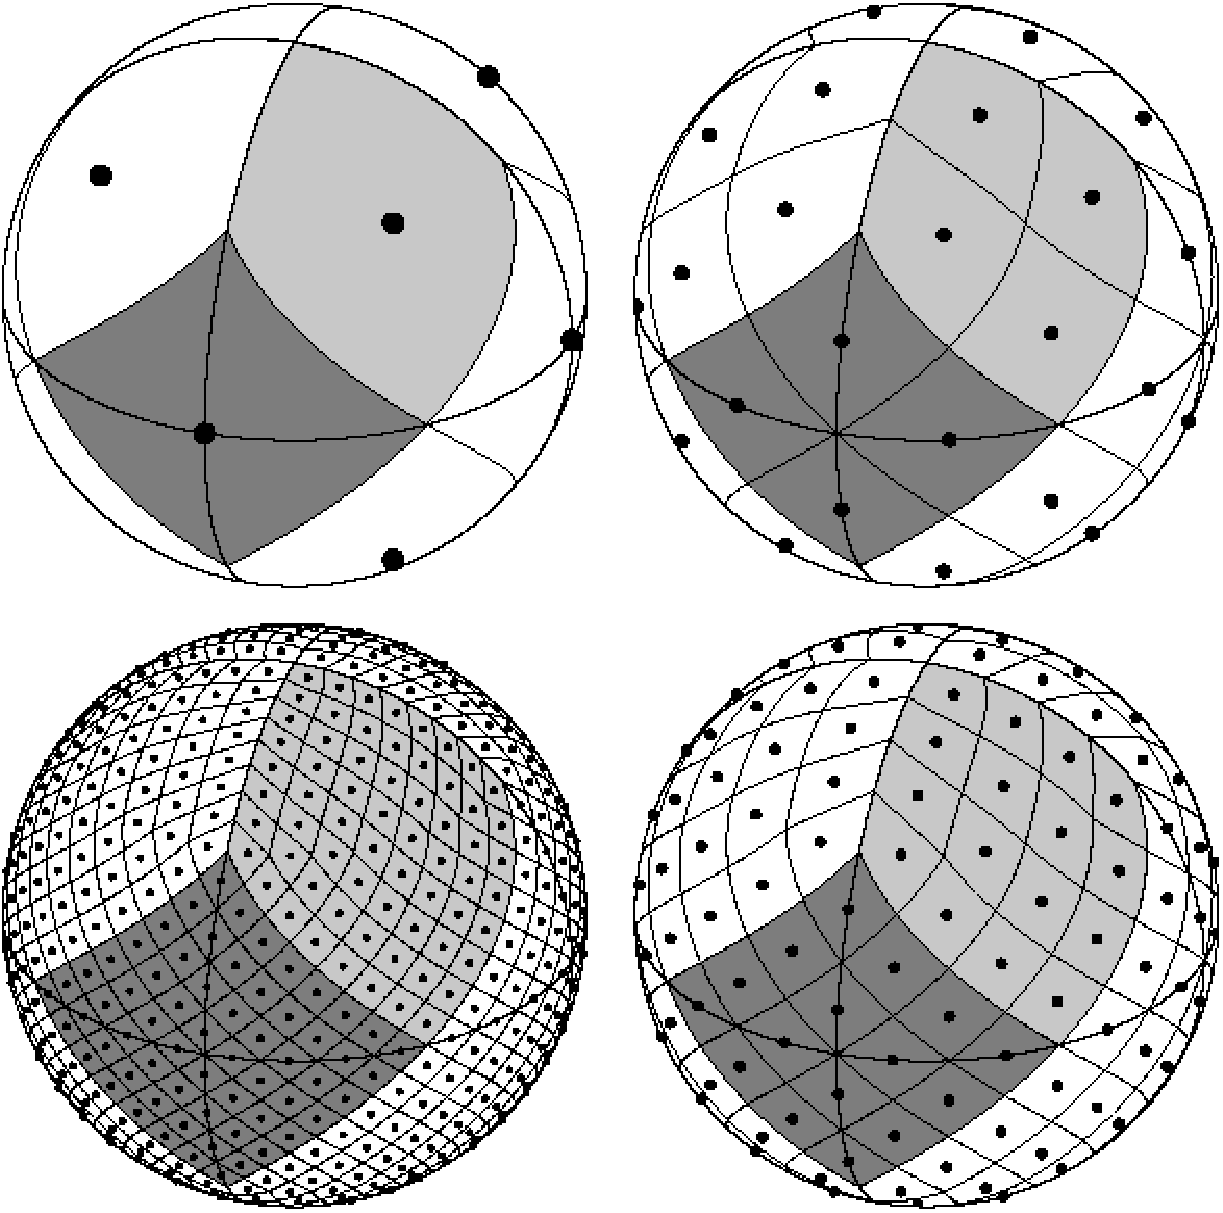
\includegraphics[height=5.5cm]{images/healpix4.pdf}}
\caption[Orthographic view of Healpix partition of the sphere]%
{\label{fig:healpix_sphere}%
Orthographic view of HEALPix partition of the sphere.}
\end{center}
\end{figure}

\begin{figure} [!ht]
\begin{center}
\centerline{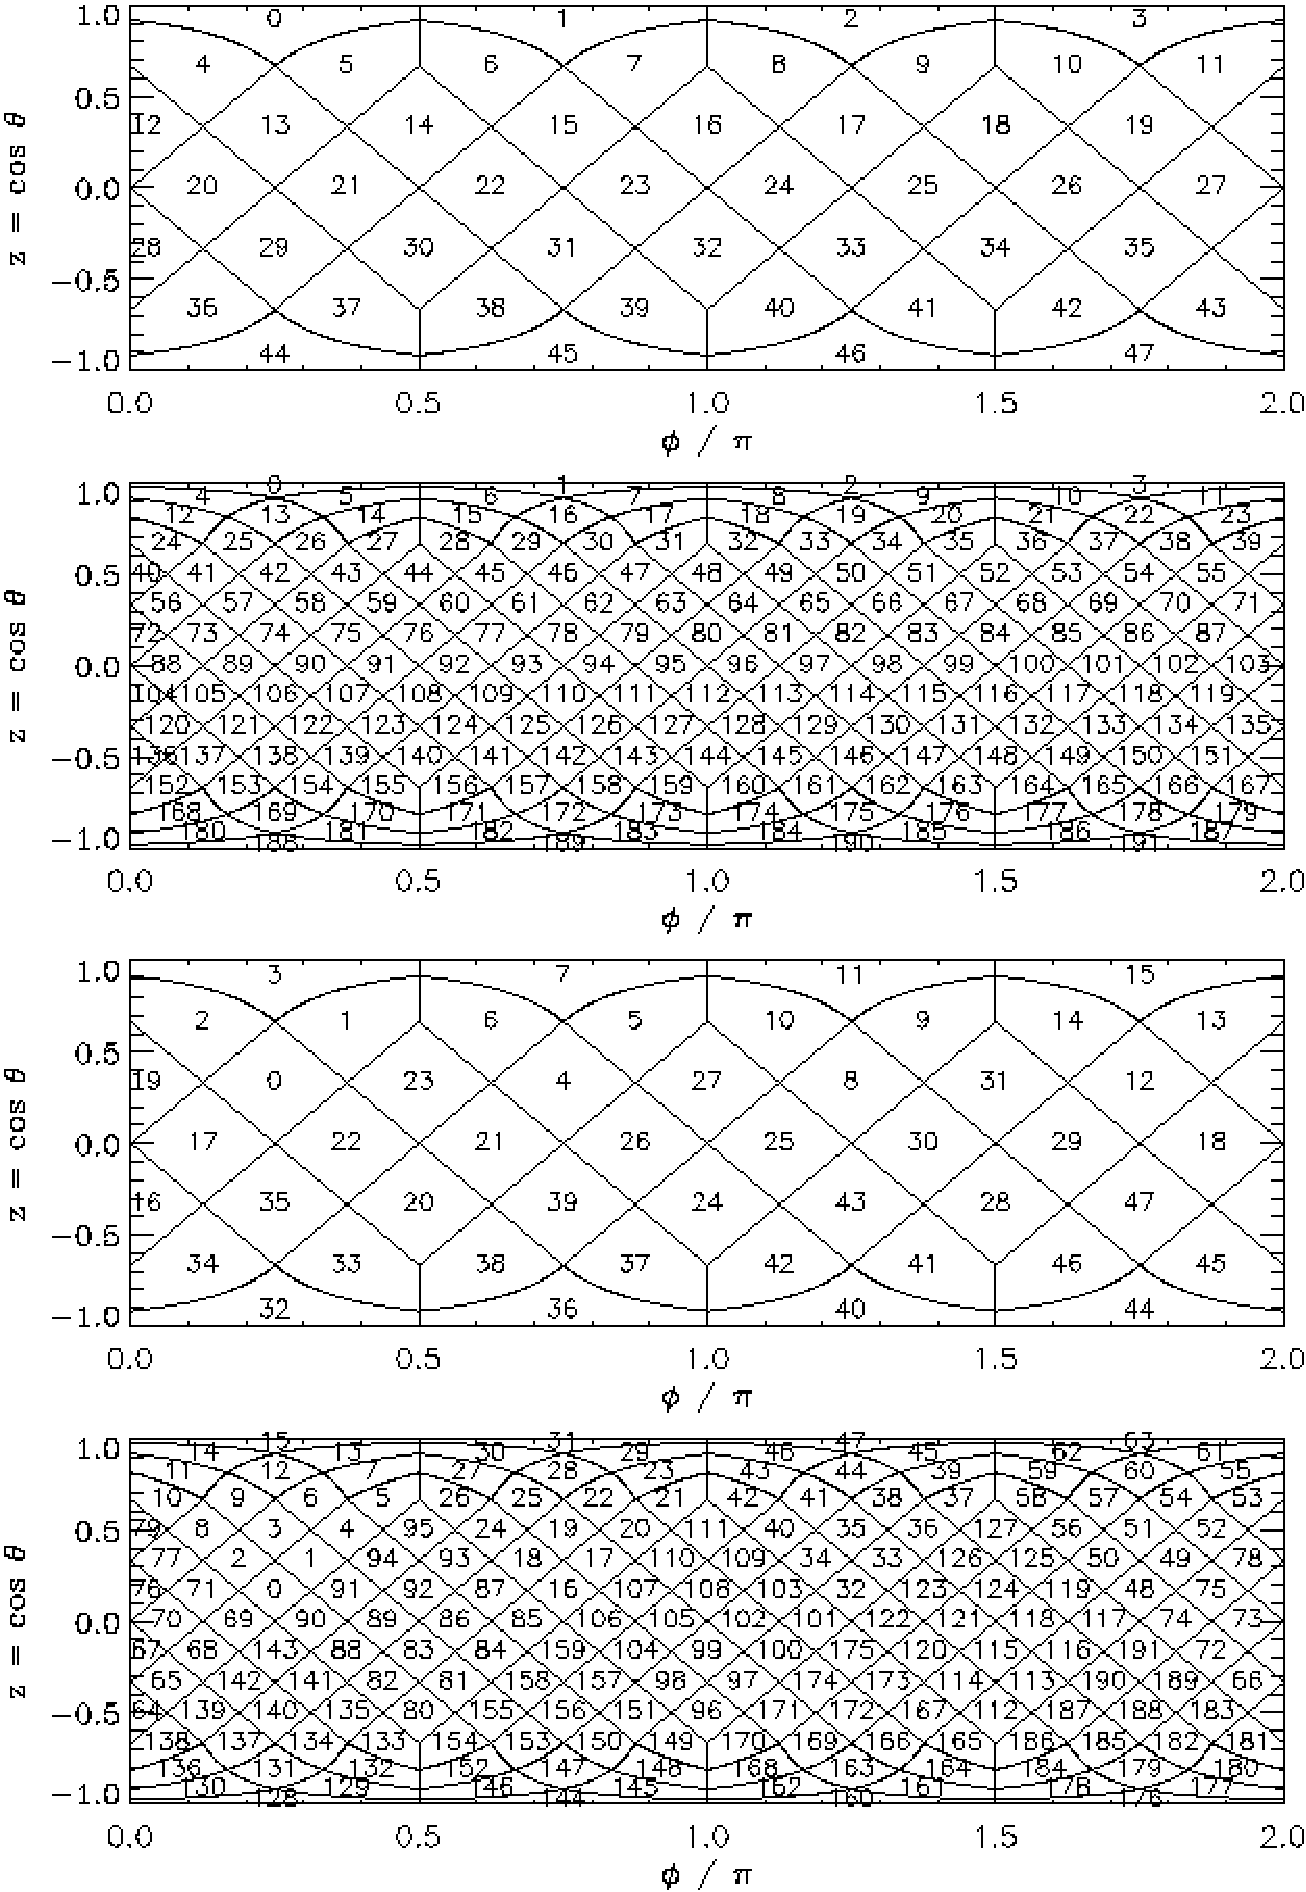
\includegraphics[height=10.5cm]{images/healpix2d.pdf}}
\caption[Cylindrical projection]%
{\label{fig:healpix_numbering}%
Cylindrical projection of the HEALPix division of a
sphere and two natural pixel numbering schemes (RING and NESTED). 
Both numbering schemes map the two dimensional 
distribution
of discrete area elements on a sphere into the one dimensional, 
integer pixel number array.
}
\end{center}
\end{figure}
\subsection{Rank-1 POVMs implementation}
\subsubsection{Measurement in classical simulation protocol}
\subsubsection{Measurement in quantum circuit model}
\subsection{Prepare-and-measure simulations}
\subsubsection{Classical transmission of one qubit}
\subsubsection{Quantum circuit counterpart}
Peres \cite{peres1995}

\begin{equation}
B_{\mu} = \ket{v_{\mu}} \bra{v_{\mu}}
\end{equation}

\begin{equation}
\ket{w_{\mu}} := \ket{v_{\mu}} + \sum_{s=d_{Q}+1}^{N} c_{\mu s} \ket{u_{\mu}}
\end{equation}

\begin{equation}
\bra{w_{\lambda}} \ket{w_{\mu}} := \bra{v_{\lambda}} \ket{v_{\mu}} + \sum_{s=d_{Q}+1}^{N} c_{\lambda s}^{\star} c_{\mu s} = \delta_{\lambda \mu}
\end{equation}

\begin{equation}
\sum_{i=1}^{n} v_{\lambda i}^{\star} v_{\mu i} + \sum_{s=d_{Q}+1}^{N} c_{\lambda s}^{\star} c_{\mu s} = \delta_{\lambda \mu}
\end{equation}

\begin{equation}
\sum_{\mu=1}^{N}\ket{v_{\mu}}\bra{v_{\mu}} = \sum_{\mu=1}^{N} B_{b,\mu} = \mathbb{1}
\end{equation}


\begin{equation}
\sum_{\mu=1}^{N}v_{\mu i}^{\star} v_{\mu j} = \delta_{ij}
\end{equation}

\begin{equation}
M = 
\begin{pmatrix}
v_{\alpha 1} & \dots & v_{\alpha d_{Q}} & c_{\alpha,d_{Q}+1} & \dots & c_{\alpha N} \\
v_{\beta 1} & \dots & v_{\beta d_{Q}} & c_{\beta,d_{Q}+1} & \dots & c_{\beta N} \\
\vdots &  & \vdots & \vdots &  & \vdots \\
v_{N1} & \dots & v_{Nd_{Q}} & c_{N,d_Q+1} & \dots & c_{NN}
\end{pmatrix}    
\end{equation}

\[\mathcal{H}^{d_Q}\ \mathcal{K}^{N}\]
\subsection{Entanglement simulations}
\subsubsection{Bell singlet state with projective measurements}
\subsubsection{CHSH inequality}
\newpage
\section{Results}\label{section:results}
\cite{software2023}\\
\textit{Random states verification}\\
\textit{Convergence plots, classical vs. quantum vs. theoretical probabilities}\\
\textit{Kullback-Leibler divergence}\\
\textit{Total variational distance}\\
\textit{CHSH inequality}
\section{Conclusion}
\textit{TBW}
\section{Acknowledgements}
We would like to express our sincere gratitude to our supervisor, Gael Sent\'is, for his guidance, support, and encouragement throughout this project. We are also grateful to the faculty and staff of the Quantum Engineering Postgraduate degree program at Universitat Polit\`ecnica de Catalunya (UPC), Universitat Aut\`onoma de Barcelona (UAB) and Institut de Ci\`encies Fot\`oniques (ICFO), for the excellent education they have provided throughout this degree. Thank you all for your support, encouragement, and guidance, without which this project would not have been possible.

\newpage
\printbibliography[heading=bibintoc, title={References}]
\newpage
\begin{appendices}
\section{Source Code Listings}\label{section:source}
\begin{minted}[
frame=lines,
framesep=2mm,
baselinestretch=1.2,
fontsize=\footnotesize,
breaklines
]{python}
import numpy as np
import cmath
import math

X = np.array([[0, 1], [1, 0]])
Y = np.array([[0, -1.j], [1j, 0]])
Z = np.array([[1, 0], [0, -1]])


class Qubit:
    def __init__(self, ket=np.array([1, 0])):
        """
        Initializes a qubit in the computational basis. If no arguments are provided, it returns the zero state.

        Parameters
        ---------
        ket : ndarray
            The qubit components in the computational basis in a 1-d complex array.
        """
        self.alpha = complex(ket[0])
        self.beta = complex(ket[1])
        self.normalize()

    def __repr__(self):
        return '{} |0> + {} |1>'.format(self.alpha, self.beta)

    def ket(self):
        return np.array([self.alpha, self.beta], dtype=np.complex_)

    def normalize(self):
        arr = self.ket()
        self.alpha, self.beta = arr/np.linalg.norm(arr)

    def rho(self):
        """
         Returns the density matrix corresponding to the qubit in a pure state.

         Returns
         -------
         ndarray
             A 2x2 density matrix corresponding to the qubit in a pure state.
         """
        return np.outer(self.ket(), self.ket().conj())

    def bloch_angles(self):
        """
        Returns the spherical coordinates of the qubit in the Bloch sphere, with polar and azimuthal angles in radians.

        Returns
        -------
        (float, float)
            The Bloch sphere coordinates, first the polar angle and then the azimuthal angle (both in radians).
        """
        r0, phi0 = cmath.polar(self.alpha)
        r1, phi1 = cmath.polar(self.beta)
        theta = 2 * math.acos(r0)
        phi = phi1 - phi0

        return theta, phi

    @staticmethod
    def density2bloch(rho):
        """
        Returns the cartesian coordinates of the specified qubit state in the Bloch sphere.

        Parameters
        ---------
        rho : ndarray
            The qubit state in density matrix form

         Returns
         -------
         (float, float, float)
             The cartesian coordinates of the qubit in the Bloch sphere (xyz).

        """
        # cast complex to real to avoid throwing ComplexWarning, imaginary part should always be zero
        return [np.real(np.trace(np.matmul(rho, sigma))) for sigma in np.array([X, Y, Z])]

    def bloch_vector(self):
        """
         Returns the cartesian coordinates of the qubit in the Bloch sphere.

         Returns
         -------
         (float, float, float)
             The cartesian coordinates of the qubit in the Bloch sphere (xyz).

         """
        return Qubit.density2bloch(self.rho())
\end{minted}
\end{appendices}
\end{document}
